\documentclass{article}
\usepackage{graphicx}
\usepackage{fancyhdr}
\pagestyle{fancy}
\lhead{Ruicheng Wu}
\rhead{07/25/2017}
\chead{Homework 10}

\begin{document}
1.

a)

Assume that G has no cycle, and consider the longest path P in G.
Let v be one of the endpoint vertex in P — since v has degree at least 2, it must have at least two edges $e_1$ and $e_2$(or more like $e_3...e_n$) incident on it.

Let $e_1$ be the last edge of the path P. Then $e_2$ and other edges cannot be incident on any other vertex of P since that would create a cycle. So $e_2,e_3...e_n$ are not part of P, and can be appended to P to give a strictly longer path. Because of this contradicts our choice of P. This would be the same if we choose another endpoint or choose both 

It is contradiction,hence G must contain a cycle.

b)

proof of a) can be rightfully applied to prove this.Since it is a graph,and there must be a longest path existing.And given every vertex with at least 2 degree, that can be conducted as both endpoints have at least 2 degree,we can exactly use the same contradiction to prove there is cycle.

2.

According to definition, a perfect matching of $K_{n,n}$ can be informally conducted as the number of ways to partition the $2n$ vertices into n sets of two vertices each:

It is generally a multinomial case(or say labelled balls in unlabelled bins): $C(2n;a_1,a_2...a_n)= \frac{2n!}{(2!)^n*n!}$,where $A(n)={2,2,2,2...2}$ with n terms.

3.

a)

min-cut={s,b}

The capacity of min-cut is 4, since $$d(s->a)=1,d(b->f)=3$$

b)
The max flow is not unique,the value of this flow is 4 as it is equal to the capacity of min-cut.

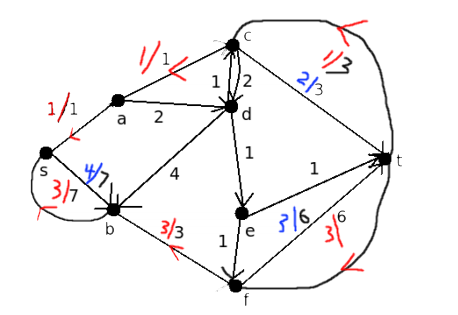
\includegraphics[scale=0.8]{HW10_3.png}

4.

a)

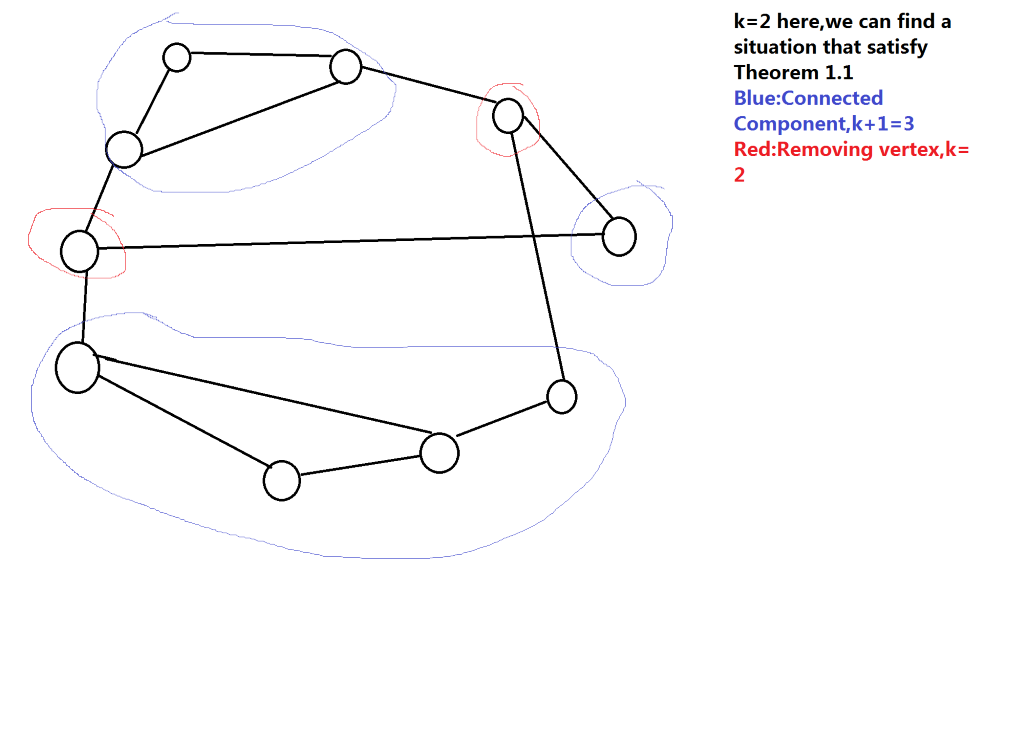
\includegraphics[scale=0.6]{HW10_4.png}

b)
Graph is on next page: 

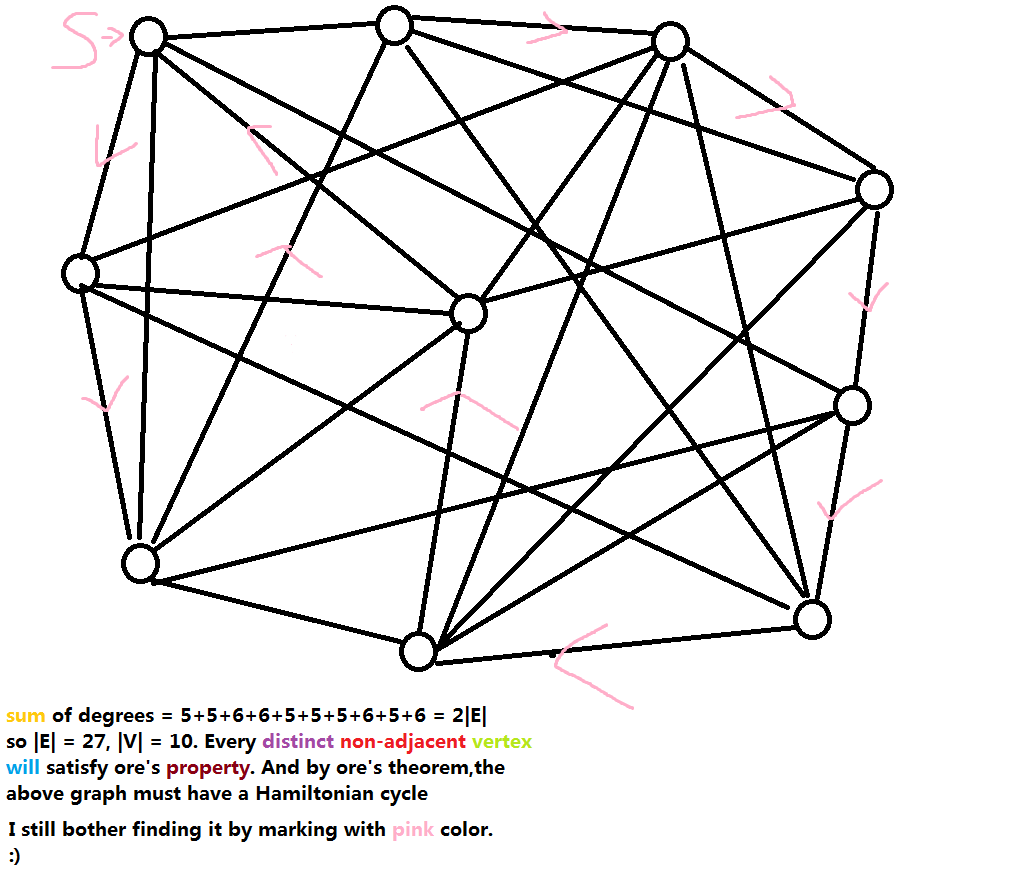
\includegraphics[scale=0.5]{HW10_4b.png}
\end{document}